\section*{Attention} 
\textit{Instead of compressing the whole sequence into a vector, determine where to look}
\subsection*{Self attention}
\textbf{Gating function:} Given query $\pmb\xi\in\mathrm R^n$ and values $\mathbf x^t\in\mathrm R^m$, \\$f_\phi(\pmb\xi, (\mathbf x^1,...,\mathbf x^s))=\frac{1}{\sum_j \exp[\phi(\pmb\xi,\mathbf x^j)]}\begin{bmatrix} \exp[\phi(\pmb\xi,\mathbf x^1)] \\...\\ \exp[\phi(\pmb\xi,\mathbf x^s)] \end{bmatrix}$\\
Simplest choice for similarity function when $m=n$: $\phi(\pmb\xi,\mathbf x)=\pmb\xi\cdot\mathbf x$\\
\textbf{Transfer function:} $F(\pmb\xi, (\mathbf x^1,...,\mathbf x^s))=[\mathbf x^1 \quad ... \quad \mathbf x^s]\cdot f_\phi(\pmb\xi, (\mathbf x^1,...,\mathbf x^s))$\\
i.e. computes convex combination of inputs wrt attention weights\\
\textbf{RNN with attention (Seq2Seq):} combining ideas of encoding information relevant for the future (RNNs) and selecting what is relevant in retrospective (attention)\\
Attend to hidden state sequence $(\mathbf h_e^1,...,\mathbf h_e^s)$ of encoder with query $\pmb\xi^i$ produced as hidden states by decoder. Use this as input into decoder, which produces hidden states $(\pmb\xi^1,...,\pmb\xi^t)$ and output sequence $(\mathbf y^1,...,\mathbf y^t)$ 
%Happens during decoding. For each word in sentence, assign weights to words from input sentence.\\
\subsection*{Memory Networks}
Recurrent attention model over possibly large external memory\\
\textbf{Recursive associative recall:} Given query $\mathbf q$ (e.g. question), find best matching memory cell $i$, use its content $\mathbf m_i$ and $\mathbf x$ to generate new query - repeat
\subsection*{Transformers}
\textit{Attention is all you need}\\
\textbf{Key-Value attention map:} given KV pairs $(\mathbf x^i,\mathbf z^i)$,\\ $F(\pmb\xi,((\mathbf x^1,\mathbf z^1),...,(\mathbf x^s,\mathbf z^s)))=[\mathbf z^1\quad...\quad\mathbf z^s]\cdot f(\pmb\xi,(\mathbf x^1,...,\mathbf x^s))$\\
$\Rightarrow$ keys determine where to look, values what features to extract\\
Similarity function: $\phi(\pmb\xi,\mathbf x)=\frac{\pmb\xi\cdot\mathbf x}{\sqrt n},\quad \pmb\xi,\mathbf x\in\mathrm R^n$\\
Assuming entries sampled from standard Gaussian, this gives standard scaling. Good since softmax can be sensitive to large input values (which kills gradient and slows down learning)\\
\textbf{Multi-headed attention:} $G(\pmb\xi,(\mathbf x^t,\mathbf z^t)_{t=1}^s)=\mathbf W\begin{bmatrix}F_1(\pmb\xi,(\mathbf x^t,\mathbf z^t))\\...\\F_h(\pmb\xi,(\mathbf x^t,\mathbf z^t)) \end{bmatrix}$\\
$F_j(\pmb\xi,(\mathbf x^t,\mathbf z^t))=F(\mathbf W_j^q\pmb\xi,(\mathbf W_j^x\mathbf x^t,\mathbf W_j^z\mathbf z^t))$\\
Alt.: $\mathbf Y=\text{softmax}(\mathbf{XW}_q\mathbf W_k^T\mathbf X^T)\mathbf{XW}_v, \mathbf W_{\{q,k,v\}}\in\mathrm R^{d\times hd},\mathbf{X,Y}\in\mathrm R^{L\times d}$\\
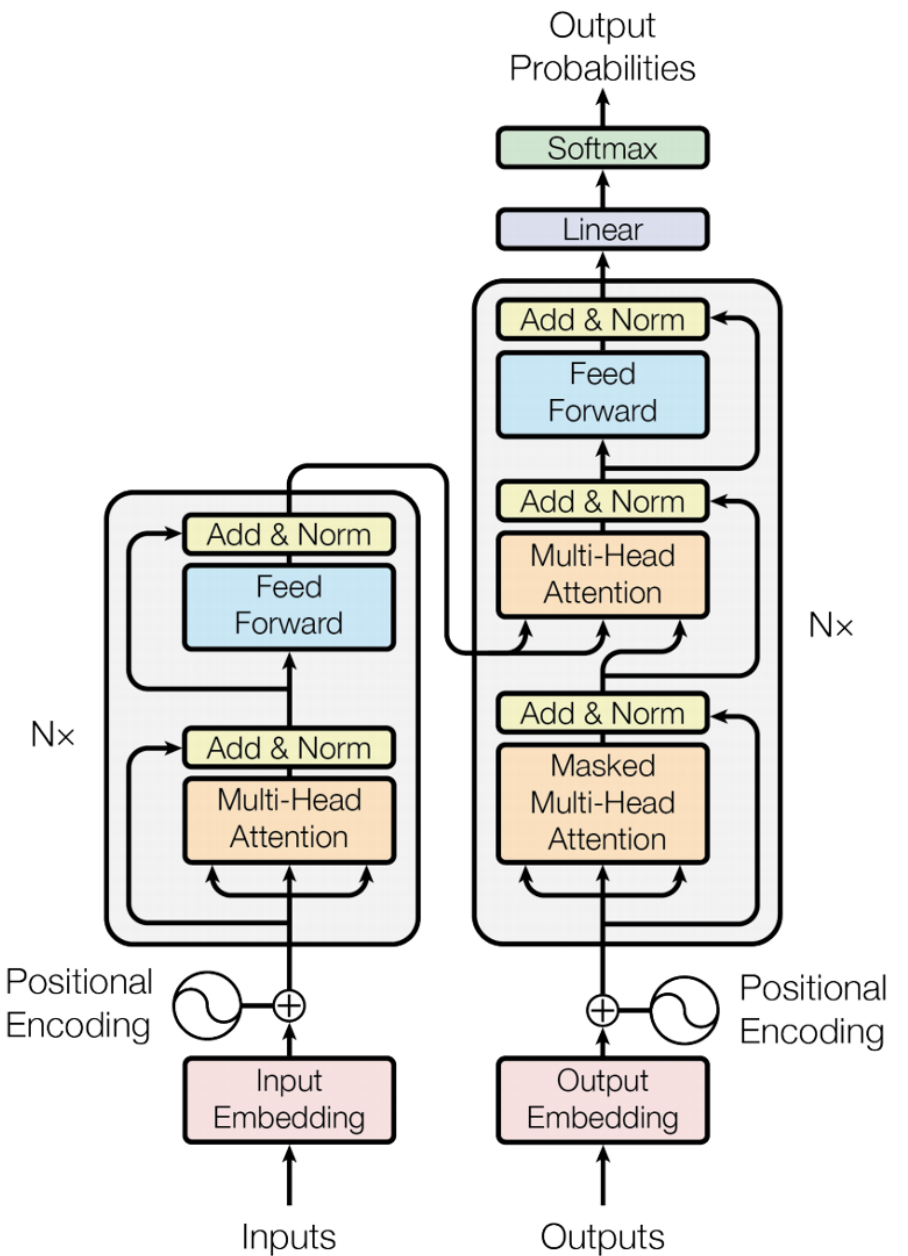
\includegraphics[scale=0.25]{transformer.png}\\
\textbf{1. Input embedding} Accounts for meaning\\
\textbf{2. Positional Encodings} Accounts for position in the input sentence. Normally use sinusoidal functions. For position $t$ and feature $k$:\\ $p_{tk}=\begin{cases} \sin(t\omega_k) \quad k \text{ even} \\ \cos(t\omega_k) \quad k \text{ odd} \end{cases} \omega_k=C^{k/n}, C=10000$\\
\textbf{3. Creating Masks} In decoder, to prevent peaking ahead.\\
\textbf{4. Multi-Head Attention Layer} Split embedding into $N$ heads and perform attention on each. Three types: Self, masked and mixed.\\
\textbf{5. Feed-Forward layer}
\subsection*{Applications in NLP}
\textit{Construct word embeddings that reflect the context}\\
\textbf{ELMo}: Input fixed embeddings on character level, build word representations with CNNs, then stack left-to-right LSTM and right-to-left LSTM. Output (for each word) is convex combination of hidden states over layers. Out-of-vocabulary (not restricted to fixed vocabulary). Train in task-specific manner.\\
\textbf{BERT}: Input sub-word unit embeddings. Leverage attention - take query and retrieve keys \& values from words in context. Insight: do not need to learn a language model. Train by word masking task - predict missing word in text. Also do next sentence prediction in pre-training. Can fine-tune for specific downstream task. \textbf{BERTology} -  representations hierarchical, struggles with negation, incomplete syntactic knowledge etc\\
\textbf{GPT-n}: Few, one or zero shot learning - add task description \& examples to working memory and let model do the rest.